\PassOptionsToPackage{unicode=true}{hyperref} % options for packages loaded elsewhere
\PassOptionsToPackage{hyphens}{url}
\PassOptionsToPackage{dvipsnames,svgnames*,x11names*}{xcolor}
%
\documentclass[10pt,]{krantz}
\usepackage{lmodern}
\usepackage{amssymb,amsmath}
\usepackage{ifxetex,ifluatex}
\usepackage{fixltx2e} % provides \textsubscript
\ifnum 0\ifxetex 1\fi\ifluatex 1\fi=0 % if pdftex
  \usepackage[T1]{fontenc}
  \usepackage[utf8]{inputenc}
  \usepackage{textcomp} % provides euro and other symbols
\else % if luatex or xelatex
  \usepackage{unicode-math}
  \defaultfontfeatures{Ligatures=TeX,Scale=MatchLowercase}
    \setmonofont[Mapping=tex-ansi,Scale=0.7]{Source Code Pro}
\fi
% use upquote if available, for straight quotes in verbatim environments
\IfFileExists{upquote.sty}{\usepackage{upquote}}{}
% use microtype if available
\IfFileExists{microtype.sty}{%
\usepackage[]{microtype}
\UseMicrotypeSet[protrusion]{basicmath} % disable protrusion for tt fonts
}{}
\IfFileExists{parskip.sty}{%
\usepackage{parskip}
}{% else
\setlength{\parindent}{0pt}
\setlength{\parskip}{6pt plus 2pt minus 1pt}
}
\usepackage{xcolor}
\usepackage{hyperref}
\hypersetup{
            pdftitle={Geometria-vectorial},
            pdfauthor={Ricardo Michel MALLQUI BAÑOS},
            colorlinks=true,
            linkcolor=Maroon,
            filecolor=Maroon,
            citecolor=Blue,
            urlcolor=Blue,
            breaklinks=true}
\urlstyle{same}  % don't use monospace font for urls
\usepackage{longtable,booktabs}
% Fix footnotes in tables (requires footnote package)
\IfFileExists{footnote.sty}{\usepackage{footnote}\makesavenoteenv{longtable}}{}
\setlength{\emergencystretch}{3em}  % prevent overfull lines
\providecommand{\tightlist}{%
  \setlength{\itemsep}{0pt}\setlength{\parskip}{0pt}}
\setcounter{secnumdepth}{5}

% set default figure placement to htbp
\makeatletter
\def\fps@figure{htbp}
\makeatother

\usepackage[spanish,es-lcroman]{babel}
\usepackage{booktabs}
\usepackage{graphicx}
\usepackage{amsmath}
\usepackage{makeidx}
\makeindex
%\usepackage{showframe}
%\usepackage[a4paper]{geometry}
%\geometry{verbose,tmargin=3cm,bmargin=3cm,lmargin=3.5cm,rmargin=3cm}

\usepackage{times}
\renewcommand{\rmdefault}{ptm}
\usepackage[lite,subscriptcorrection,nofontinfo,zswash]{mtpro2}

\usepackage{graphicx}

% Determine if the image is too wide for the page.
\makeatletter
\def\ScaleIfNeeded{%
  \ifdim\Gin@nat@width>\linewidth
    \linewidth
  \else
    \Gin@nat@width
  \fi
}
\makeatother

% Resize figures that are too wide for the page.
\let\oldincludegraphics\includegraphics
\renewcommand\includegraphics[2][]{%
  \oldincludegraphics[scale=0.85]{#2}
}

\usepackage{amsthm}
\makeatletter
\def\thm@space@setup{%
  \thm@preskip=8pt plus 2pt minus 4pt
  \thm@postskip=\thm@preskip
}
\makeatother



\flushbottom 

\frontmatter
\usepackage[]{natbib}
\bibliographystyle{apalike}

\title{Geometria-vectorial}
\author{Ricardo Michel MALLQUI BAÑOS}
\providecommand{\institute}[1]{}
\institute{Universidad Nacional San Cristóbal De Huamanga}
\date{2020-08-11}

\usepackage{amsthm}
\newtheorem{theorem}{Teorema}[chapter]
\newtheorem{lemma}{Lema}[chapter]
\newtheorem{corollary}{Corolario}[chapter]
\newtheorem{proposition}{Proposición}[chapter]
\newtheorem{conjecture}{Conjectura}[chapter]
\theoremstyle{definition}
\newtheorem{definition}{Definición}[chapter]
\theoremstyle{definition}
\newtheorem{example}{Ejemplo}[chapter]
\theoremstyle{definition}
\newtheorem{exercise}{Ejercicio}[chapter]
\theoremstyle{remark}
\newtheorem*{remark}{Observación}
\newtheorem*{solution}{Solución}
\let\BeginKnitrBlock\begin \let\EndKnitrBlock\end
\begin{document}
\maketitle

%\cleardoublepage\newpage\thispagestyle{empty}\null
%\cleardoublepage\newpage\thispagestyle{empty}\null
%\cleardoublepage\newpage
\thispagestyle{empty}
\begin{center}

\includegraphics{U.pdf}
\end{center}

%\setlength{\abovedisplayskip}{-5pt}
%\setlength{\abovedisplayshortskip}{-5pt}

{
\hypersetup{linkcolor=}
\setcounter{tocdepth}{2}
\tableofcontents
}
\listoftables
\listoffigures
\newcommand{\N}{\mathbb{N}}
\newcommand{\R}{\mathbb{R}}
\newcommand{\CC}{\mathbb{C}}
\newcommand{\I}{\mathbb{I}}
\newcommand{\f}{\mathbb{f}}
\newcommand{\X}{\mathbb{X}}
\newcommand{\D}{\mathbb{D}}
\newcommand{\Z}{\mathbb{Z}}
\newcommand{\Q}{\mathbb{Q}}
\newcommand{\norm}[1]{\left\Vert#1\right\Vert}
\newcommand{\abs}[1]{\left\vert#1\right\vert}
\newcommand{\set}[1]{\left\{#1\right\}}
\newcommand{\seq}[1]{\left<#1\right>}
\newcommand{\co}[1]{\left[#1\right]}
\newcommand{\cc}[1]{\left(#1\right)}
\newcommand{\J}{\mathcal{J}}
\newcommand{\K}{\mathcal{K}}
\newcommand{\M}{\mathcal{M}}
\newcommand{\F}{\mathcal{F}}

\hypertarget{resumen}{%
\chapter*{Resumen}\label{resumen}}


Este es un libro sobre la geometria vectorial
edicion 2

\hypertarget{introducciuxf3n}{%
\chapter*{Introducción}\label{introducciuxf3n}}


\mainmatter

\hypertarget{vectores}{%
\chapter{Vectores}\label{vectores}}

\hypertarget{intro}{%
\chapter{Rectas}\label{intro}}

\hypertarget{lugar-geomuxe9trico}{%
\chapter{Lugar geométrico}\label{lugar-geomuxe9trico}}

Here is a review of existing methods.

\hypertarget{circunferencia}{%
\chapter{Circunferencia}\label{circunferencia}}

Sea \(\vec{a}=(a_1,a_2)\) entonces el vector escalado es \(r\vec{a}\parallel\vec{a}\); el vector perpendicular a este es \(\vec{a}^\perp=(-a_2,a_1)\) la norma del vector \(\vec{a}\) es \(\left\|a\right\|=\sqrt{a_1^2+a_2^2}\) el vector unitario en la dirección de \(\vec{a}\) es \(\vec{\mu}=\frac{\vec{a}}{\left\|a\right\|}\) que es paralela a este. Dado dos puntos \(P_1\) y \(P_2\) estos definen un vector \(\vec{P_1P_2}=P_2-P_1\). Los vectores en dirección de los ejes positivos son \(i=(1,0)\) y \(j=(0,1)\); cualquier vector se pueden expresar en términos de estos es decir \(\vec{a}=(a_1,a_2)=a_1(1,0)+a_2(0,1)=a_1i+a_2j\). De acuerdo al ángulo de inclinación del vector se tiene la siguiente representación \(\vec{a}=\left\|\vec{a}\right\|(\cos\theta,\sin\theta)\). \(C\)

\BeginKnitrBlock{theorem}[russ]
\protect\hypertarget{thm:www}{}{\label{thm:www} \iffalse (russ) \fi{} }Dada el espacio \(R\) y \(r\in R\) se tiene que \(\mathcal{R}(r)=\lim_{t\to\infty}g(y)_r\)
\EndKnitrBlock{theorem}

\(\sum\)

\begin{figure}

{\centering 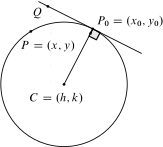
\includegraphics{circunferencia} 

}

\caption{Vector}\label{fig:C1}
\end{figure}

\begin{figure}

{\centering 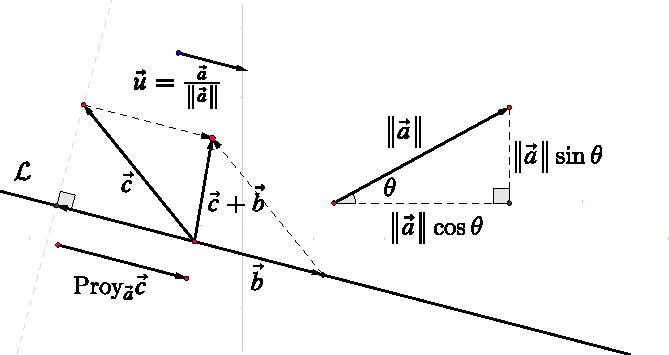
\includegraphics{vector} 

}

\caption{Circunferencia}\label{fig:C2}
\end{figure}

Dos vectores son ortogonales (\(\vec{a}\perp\vec{b}\)) si \(\left|\vec{a}-\vec{b}\right|=\left|\vec{a}+\vec{b}\right|\) y verifican

\(\left|\vec{b}\right|^2+\left|\vec{b}\right|^2+=\left|\vec{a}+\vec{b}\right|^2\)
\(\vec{a}\vec{b}=0\)
\(\vec{a}\parallel\vec{b}^\perp\)
\(\vec{a}\) y \(\vec{b}\) son LI si y solo si \(r\vec{a}+s\vec{b}=0\) implica \(r=0\) y \(s=0\).

La proyeccion de \(\vec{a}\) sobre \(\vec{b}\) es otro vector \(\text{Proy}_{\vec{b}}\vec{a}\)

\(\vec{a}=\text{Proy}_{\vec{b}}\vec{a}+\text{Proy}_{\vec{b}^\perp}\vec{a}\) si hacemos \(\vec{a}=p\vec{b}+q\vec{b}^\perp\) entonces \(q=\frac{\vec{a}\vec{b}}{\left\|\vec{b}\right\|^2}\) y \(p=\frac{\vec{a}\vec{b}^\perp}{\left\|\vec{b}\right\|^2}\) pues \(\left\|\vec{b}\right\|=\left\|\vec{b}^\perp\right\|\) entonces \(\text{Proy}_{\vec{b}}\vec{a}=\frac{\vec{a}\vec{b}}{\left\|\vec{b}\right\|^2}\vec{b}=\frac{\vec{a}\vec{b}}{\left\|\vec{b}\right\|}\frac{\vec{b}}{\left\|\vec{b}\right\|}=\text{Cp}_{\vec{b}}\vec{a}\frac{\vec{b}}{\left\|\vec{b}\right\|}\); \(\text{Cp}_{\vec{b}}\vec{a}=\frac{\vec{a}\vec{b}}{\left\|\vec{b}\right\|}\) recibe el nombre de componente de \(\vec{a}\) en la dirección de \(\vec{b}\)

Dado \(P_0\) y un vector \(\vec{a}\) entonces la recta se define como el conjunto de puntos \(\mathcal{L}=\left\{P\in\mathbb{R}^2/P=P_0+t\vec{a};\: t\in \mathbb{R}\right\}\) que recibe el nombre de ecuación vectorial de la recta. \(P\in\mathcal{L}\iff (P-P_0)\cdot\vec{a}^\perp=0\). De la ecuación vectorial de la recta se tiene si \(P=(x.y)\); \(P_0=(x_0,y_0)\) y \(\vec{a}=(a_1,a_2)\) se tiene la ecuación paramétrica de la recta. \(x=x_0+ta_1\); \(y=y_0+ta_2\) de esto se obtiene la ecuación simétrica de la recta \[\frac{x-x_0}{a_1}=\frac{y-y_0}{a_2}.\] Sea \(\vec{n}=(a,b)=\vec{a}^\perp\) entonces se tiene que si \(P\in \mathcal{L}\) entonces \((P-P_0)\cdot \vec{n}=0\) pues son perpendicualres; entonces \(P\cdot \vec{n}=P_0\cdot \vec{n}\iff ax+by=-c\implies ax+by+c=0\) que recibe el nombre de ecuación general de la recta. Sea \(Q=(x_1,y_1)\) un punto exterior a \(\mathcal{L}\) entonces la distancia de \(Q\) a \(\mathcal{L}\) se define como

\begin{align*}d[Q;\mathcal{L}] & =\left|\text{Cp}_{\vec{n}}(Q-P_0)\right| \\
& =\left|\frac{(Q-P_0)\cdot\vec{n}}{\left|\vec{n}\right|}\right| \\
& =\left|\frac{Q\cdot\vec{n}-P_0\cdot\vec{n}}{\left|\vec{n}\right|}\right| \\
& =\frac{\left|ax_1+by_1+c\right|}{\sqrt{a^2+b^2}}
\end{align*}

Sean \(\mathcal{L}_1\) y \(\mathcal{L}_2\) dos rectas; con vectores directores \(\vec{a}=(a_1,a_2)\) y \(\vec{b}=(b_1,b_2)\) respectivamente; entonces \(\mathcal{L}_1\cap\mathcal{L}_2=(d_1,d_2)\) donde \(d_1\) y \(d_2\) satisfacen el sistema generado por las ecuaciones generales de \(\mathcal{L}_1\) y \(\mathcal{L}_2\); \(a_1x+a_1y+k_1=0\) y \(b_1x+b_1y+k_2=0\).

La pendiente de una recta se deduce de su vector director es decir si \(\vec{a}=(a_1,a_2)\) entonces \(m=\frac{a_2}{a_1}\); de esto se deduce \(\vec{a}=(a_1,a_2)=a_1(1,\frac{a_2}{a_1})=a_1(1,m)\). El angulo generado por las \(\mathcal{L}_1\) con pendiente \(m_1\) y \(\mathcal{L}_2\) con pendiente \(m_1\); está dada por \(\theta=\arctan\left(\frac{m_1-m_2}{1+m_1m_2}\right)\).

El círculo se define como el conjunto de punto \(P=(x,y)\) que satisfacen la ecuación \[\left \|P-C\right\|=r\] \(r>0\) es el radio, \(C=(h,k)\) es el centro entonces la ecuación del círculo es \[\left \|P-C\right\|=r\iff (x-h)^2+(y-k)^2=r^2.\]

La ecuación de la recta tangente en \(P_0=(x_0,y_0)\) (\(P=P_0\) en el gráfico) está dada por \[(Q-P_0)\cdot(P_0-C)=0\] donde \(Q=(x,y)\neq P\) cualquiera; entonces \[(Q-P_0)\cdot(P_0-C)=0\iff  (x-x_0,y-y_0)(x_0-h,y_0-k)=0\] lo cual es equivalente a \[(x-h)(x_0-h)+(x-k)(y_0-k)=r^2\]

\hypertarget{paruxe1bola}{%
\chapter{Parábola}\label{paruxe1bola}}

Sean la recta \(\mathcal{L}\) y el punto \(F\) fijos; los puntos \(P\) que satisfacen la ecuación

\begin{equation} 
d\left[P;F\right]=d\left[P;\mathcal{L}\right]=\left|p\right|\label{eq:www}
\end{equation}

generan una curva llamada \emph{parábola}, la excentricidad es el cociente de estas dos distancias que es igual a \(1\) pues ambas son iguales a \(\left|p\right|\).

\(\mathcal{L}\) es la \emph{recta directriz} cuya ecuación es \(x'=-p\) en el sistema \(X'Y'\); \(F\) es el \emph{foco}, \(V=(h,k)\) el \emph{vertice}; \(p\) es el parámetro de la parábola; y \(RR'\) el \emph{lado recto} de la parábola.

\begin{figure}

{\centering 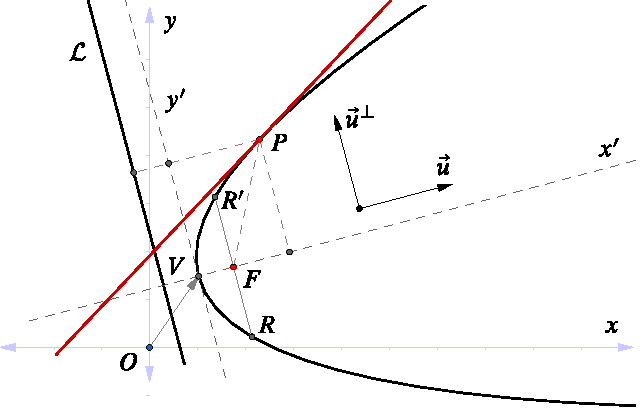
\includegraphics{parabola} 

}

\caption{Prábola}\label{fig:hiperbola1}
\end{figure}

Los puntos \(P\) en el sistema \(X'Y'\) satisfacen
\(P=(x,y)=V+x'\vec{u}+y'\vec{u}^\perp\) de donde al despejar \(x'\) e \(y'\) resultan \(x'=[(x,y)-V]\vec{u}\) e \(y'=[(x,y)-V]\vec{u}^\perp\)
la recta directriz en el sitema \(X'Y'\) es
\(\mathcal{L}=\left\{Q/Q=(V-p\vec{u})+t\vec{u}^\perp,\:t\in \mathbb{R}\right\}\); donde el vértice es \(F=V+p\vec{u}\) luego se tiene las ecuaciónes

\begin{equation}
d[P;\mathcal{L}]=\left|\text{Cp}_{\vec{u}}\vec{PQ}\right|=\left|(Q-P)\cdot\vec{u}\right|=\left|x'+p\right|\label{eq:1w}
\end{equation}

\begin{equation}
d[P;F]=\left|P-F\right|=\left|(x'-p)\vec{u}+y'\vec{u}^{\perp}\right|\label{eq:2w}
\end{equation}

por lo tanto reemplazando \eqref{eq:1w} y \eqref{eq:2w} en \eqref{eq:www}
\begin{align*}
d\left[P;F\right]^2=d\left[P;\mathcal{L}\right]^2
& \implies \left|(x'+p)\vec{u}+y'\vec{u}^\perp\right|^2=\left|x'+p\right|^2 \\
&\implies (x'-p)^2+y'^2=(x'+p)^2\\
&\implies y'^2=4px'
\end{align*}

De este modo \(P\in\mathcal{P}\) si \(P\) satisface la \emph{ecuacion vectorial} de \(\mathcal{P}\) \[P=(x,y)=V+x'\vec{u}+y'\vec{u}^\perp;\: \text{donde } y'^2=4px'; \:\left|\vec{u}\right|=1\]

Cuando el eje es paralelo al eje \(x\); se tiene \(\vec{u}=i=(1,0)\) entonces \[(x,y)=V+x'\vec{u}+y'\vec{u}^\perp=(h+x',k+y')\] implica \(x'=x-h\) y \(y'=y-k\) en \(y'^2=4px'\) resulta \((y-k)^2=4p(x-h)\) (\(y^2=4px\) si \(V\) está en el origen); entonces \(F=V+p\vec{u}=(h+p,k)\); \(\mathcal{L}: x=h-p\). Si \(p<1\) la parábola se invierte simétricamente a la directriz.

Cuando el eje es paralelo al eje \(y\); \(\vec{u}=j=(0,1)\) entonces \[(x,y)=V+x'\vec{u}+y'\vec{u}^\perp=(h-y',k+x')\] implica \(x'=y-k\) y \(y'=h-x\) en \(y'^2=4px'\) resulta \((x-h)^2=4p(y-k)\) (\(x^2=4py\) si \(V\) está en el origen); entonces \(F=V+p\vec{u}=(h,k+p)\); \(\mathcal{L}: x=k-p\). Si \(p<1\) la parábola se invierte simétricamente a la directriz.

\BeginKnitrBlock{theorem}[Ecuaciones de la recta tangente de una parábola]
\protect\hypertarget{thm:unnamed-chunk-1}{}{\label{thm:unnamed-chunk-1} \iffalse (Ecuaciones de la recta tangente de una parábola) \fi{} }La ecuación de la recta tangente a \(y^2=4px\) en el punto \(P_0=(x_0,y_0)\) está dada por
\begin{equation}
y=\frac{2p}{y_0}(x+x_0)
\label{eq:w1}
\end{equation}
y la ecuación de la recta tangente a \((y-k)^2=4p(x-h)\) en el punto \(P_0=(x_0,y_0)\) está dada por
\begin{equation}
(y_0-k)(x_0-k)=4p\left[\left(\frac{x+x_0}{2}-h\right)\right]
\label{eq:w2}
\end{equation}
similarmente la ecuación de la recta tangente a \((x-h)^2=4p(y-k)\) en el punto \(P_0=(x_0,y_0)\) está dada por
\begin{equation}
(x_0-h)(x_0-h)=4p\left[\left(\frac{y+y_0}{2}-h\right)\right].
\label{eq:w3}
\end{equation}
\EndKnitrBlock{theorem}

\BeginKnitrBlock{proof}
\iffalse{} {Demostracion. } \fi{}En efecto sea \ldots{}
\EndKnitrBlock{proof}

\BeginKnitrBlock{exercise}
\protect\hypertarget{exr:unnamed-chunk-3}{}{\label{exr:unnamed-chunk-3} }Al realizarse una transformacion de coordenadas, el eje de una parabola \(\mathcal{P}\) resulta orientada segun el vector \((3,4)\). En \(X'Y'\) un punto \(Q'=(20,-20)'\in\mathcal{P}\) en els sistema \(xy\) el foco de \(\mathcal{P}\) \(E=(11,5)\). Determinar en el sistema \(xy\) un punto \(R\) de la parabola \(\mathcal{P}\) tal que el trinagulo \(QVR\) sea rectangulo en \(V\) vertice de la parábola.
\EndKnitrBlock{exercise}

\BeginKnitrBlock{exercise}
\protect\hypertarget{exr:unnamed-chunk-4}{}{\label{exr:unnamed-chunk-4} }La circunferencia \(\mathcal{C}=(x-3)^2+(y-3)^2=25\) es tangente a una parábola \(\mathcal{P}\) en \(P_0=(x_0,y_0)\), \(y_0>7\). La recta \(\mathcal{L}:4x-3y+12=0\) es normal a \(\mathcal{P}\) y \(\mathcal{C}\) en \(P_0\) y corta al eje focal de \(\mathcal{P}\) en el punto \(R\). Si \(\left|\vec{C_0P_0}\right|=\left|\vec{P_0R}\right|\) y si la distancia \(d[P_0; \text{eje focal}]=4\), hallar la ecuación de la parábola \(\mathcal{P}\). \(C_0\) es el centro de la circunferencia y la absisa del vértice es menor que 6.
\EndKnitrBlock{exercise}

\BeginKnitrBlock{solution}
\iffalse{} {Solución. } \fi{}\(P_0=C_0\pm r\vec{u}_{\mathcal{L}}\) donde \(r=5\), \(C_0=(3,8)\) y \(\vec{u}_{\mathcal{L}}=\frac{(3,4)}{5}\) es decir \(P_0=(3,8)\pm 5\frac{(3,4)}{5}\) de esto consideramos \(P_0=(x_0,y_0)=(6,12)\) por condición del problema con esto la recta tangente a \(\mathcal{C}\) y \(\mathcal{P}\) es \(\mathcal{L}_T:(x,y)(3,4)=(3,4)(6,12)\) equivalentemente \(\mathcal{L}_T:3x+4y=66\).

Ya que \(\left|\vec{C_0P_0}\right|=5=\left|\vec{P_0R}\right|\) y \(d[P_0;\text{eje focal}]=d[P_0; Q]=4\) entonces el triángulo \(P_0QR\) es un triángulo rectángulo notable, por lo tanto \(\left|\vec{QR}\right|=3\) por el Teorema de Pitágoras, además \(\vec{P_0R}=\vec{P_0Q}+\vec{QR}\) es decir si \(\vec{P_0Q}=(v_1,v_2)\) se tiene la ecuacion \((3,4)=4(v_1,v_2)\pm 3(-v_2,v_1)\) que al resolverla se tiene \(\vec{P_0R}=(v_1,v_2)=(1,0)\) o \(\vec{P_0R}=(v_1,v_2)=\left(\frac{24}{25},\frac{7}{25}\right)\) entonces \(Q=P_0+4(0,1)=(6,16)\) o \(Q=P_0+4\left(\frac{24}{25},\frac{7}{25}\right)=\left(6+\frac{96}{25},12+\frac{28}{25}\right)\) esto indica considerar \(Q=(6,16)\) pues el vertice (tiene absisa menor que 6), debe estar a la derecha de \(P_0\) pues la recta \(\mathcal{L}_T\) tiene pendiente negativa. Por lo tanto \(\mathcal{L}_T\cap \mathcal{F}:x=16=(\frac{2}{3},16)\) y por propiedad de la tangente a una parábola se tiene el vértice \(V=\left(\frac{\mathcal{L}_T\cap \mathcal{F}+Q}{2}\right)=\left(\frac{10}{3}, 16\right)\). La ecuación de la parabola en le sistema original es \((y-h)^2=4\rho(x-k)\) donde \((h,k)=\left(\frac{10}{3}, 16\right)\) y \((6,12)\in\mathcal{P}\) se tiene \((-4)^2=4\rho(8/3)\) de donde \(\rho=\frac{3}{2}\) entonces la recta directriz pasa por \(\left(\frac{10}{3}, 16\right)+\frac{3}{2}(1,0)=\left(\frac{7}{3}, 16\right)\) por tanto \(\mathcal{L}_D:x=\frac{7}{3}\) y la ecuacion de la parábola es \[(y-16)^2=4\rho\left(x-\frac{10}{3}\right)\] por ser paralela al eje \(x.\)
\EndKnitrBlock{solution}

\BeginKnitrBlock{exercise}
\protect\hypertarget{exr:unnamed-chunk-6}{}{\label{exr:unnamed-chunk-6} }Los puntos \(A=(60,13)\) y \(B=(-4,61)\) estan sobre una parábola \(\mathcal{P}\) además son simétricos con recpecto al eje focal. Desde un punto \(Q\) sobre el eje focal se traza un recta tangente a \(\mathcal{P}\) que pasa por \(B,\) hallar la ecuación de \(\mathcal{P}\) y las ecuaciones de las rectas tangentes trazadas desde \(Q\).
\EndKnitrBlock{exercise}

\BeginKnitrBlock{solution}
\iffalse{} {Solución. } \fi{}Ya que \(A\) y \(B\) son simétricas entonces \(P_0=\frac{A+B}{2}=(28,37) \in \mathcal{L}_F\) donde \(\mathcal{L}_F\) es el eje focal paralelo al vector \(\vec{AB}^\perp=(B-A)^\perp=(-64,48)\parallel(-4,3)=\vec{v}_L\) es decir \(\vec{v}_F\) y \(P_0\) nos genera la ecuación del eje focal \(\mathcal{L}_F:4x+3y=1\). De otro lado dado el punto \(Q=(20,x)\in\mathcal{L}_F\) que al reemplazarlo en la recta del eje focal nos genera \(x=-27\) de donde \(Q=(20,-27)\) ademas el vértice de la parabola es \(V=\frac{Q+P_0}{2}=(4,5)\) por propiedad.

Con el objetivo de hallar el valor de \(\rho\) en la ecuación \(y'^2=4\rho x'\) se halla las coordenadas de \(B\) en el nuevo sistema de coordenadas centrada en \(V\) con vector director \(\vec{u}=\frac{(3,4)}{5}\), haciendo uso de la relación \[(x,y)=V+x'\vec{u}+y'\vec{u}^\perp\] se obtiene \(x'=\left[B-V\right]\vec{u}=40\) y \(y'=\left[B-V\right]\vec{u}^\perp=40\) por tanto reemplazando \(B=(-4,61)=(40,40)'\) en \(y'^2=4\rho x'\) se tiene que \(\rho=10\)

Los vectores directores de las rectas tangentes en el sistema \(X'Y'\) son \((2,1)\) y \((2,-1)\) respectivamente por tanto sus ecuaciones son \(\mathcal{L}_A: 2y'=x'+40\) y \(\mathcal{L}_B=-2y'=x'+40\) estas ecuaciones en el sistema original con \(x'=\left[(x,y)-(4,5)\right]\frac{(3,4)}{5}\) y \(y'=\left[(x,y)-(4,5)\right]\frac{(-4,3)}{5}\) reemplazadas resultan \(\mathcal{L}_A:2y-11x-166=0\) y \(\mathcal{L}_B:5x-10y-170=0\)
\EndKnitrBlock{solution}

\begin{enumerate}
\def\labelenumi{\arabic{enumi}.}
\tightlist
\item
  ww
\end{enumerate}

\hypertarget{elipse}{%
\chapter{Elipse}\label{elipse}}

Dados dos puntos distintos \(F_1\) y \(F_2\) llamados focos; la elipse\index{elipse} \(\mathcal{E}\) es el conjunto formado por los puntos \(P\) que satisfacen la ecuacion
\begin{equation} 
\left|P-F_1\right|+\left|P-F_2\right|=2a
\label{eq:binom}
\end{equation}
\(C=(h,k)\) es el centro de la elipse; \(x'\) eje focal, \(V_1\) y \(V_2\) son los vértices de la elipse; \(\overline{V_1V_2}\) el eje mayor \(\overline{RR'}\) el lado recto; \(\overline{B_1B_2}\) el eje menor de longitud \(2b\). En el sistema \(X'Y'\) se tiene \(B_1=(0,b)'\); \(B_2=(0,-b)'\); \(F_1=(-c,0)'\); \(F_2=(c,0)'\) y \(C=(0,0)'\).

\begin{figure}

{\centering 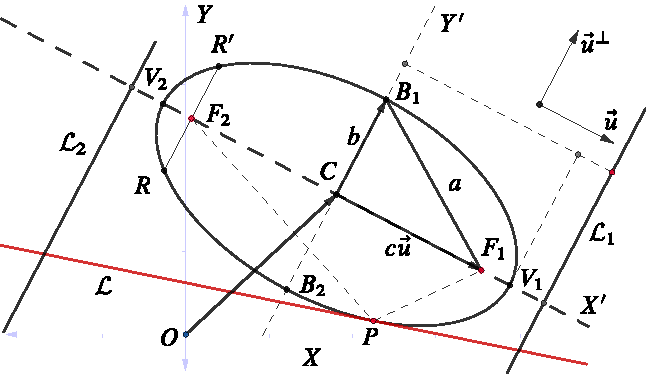
\includegraphics{elipse} 

}

\caption{Elipse}\label{fig:pressure1}
\end{figure}

Dado \(P\in \mathcal{E}\), la excentricidad \(e\) se define como
\begin{equation}
\frac{d\left[P;F_1\right]}{d\left[P;\mathcal{L}_1\right]}=e=\frac{d\left[P;F_2\right]}{d\left[P;\mathcal{L}_2\right]}
\label{eq:ww}
\end{equation}
\(d\left[B_i;F_1\right]=d\left[B_i;F_2\right]= a\) y \(d\left[V_i;C\right]=d\left[V_i;C\right]=a\), \(i=1,2\).

\BeginKnitrBlock{theorem}
\protect\hypertarget{thm:unnamed-chunk-8}{}{\label{thm:unnamed-chunk-8} }En la elipse se verifican las siguientes igualdades

\begin{enumerate}
\def\labelenumi{\arabic{enumi}.}
\item
  \(d\left[B_1;F_i\right]=d\left[B_2;F_i\right]=a\)
\item
  \(d\left[V_1;C\right]=d\left[V_2;C\right]=a\)
\item
  \(d\left[C;\mathcal{L}_1\right]=d\left[C;\mathcal{L}_2\right]=\frac{c}{e}\)
\item
  \(c=d\left[P;F_1\right]=d\left[P;F_2\right]\implies c=ae\)
\end{enumerate}
\EndKnitrBlock{theorem}

\BeginKnitrBlock{proof}
\iffalse{} {Demostracion. } \fi{}
1. Ya que \(d\left[B_1;F_1\right]+d\left[B_1;F_2\right]=2a=d\left[B_2;F_1\right]+d\left[B_2;F_2\right]\) es decir \(2d\left[B_1;F_i\right]=2a=2d\left[B_2;F_i\right]\) entonces \(d\left[B_1;F_i\right]=a=d\left[B_2;F_i\right]\) \(i=1,2\).

\begin{enumerate}
\def\labelenumi{\arabic{enumi}.}
\setcounter{enumi}{1}
\item
  Por la definición \eqref{eq:binom} de la elipse se tiene
  \begin{equation}
  d\left[V_1;F_2\right]+d\left[V_1;F_1\right]=2a
  \label{eq:er}
  \end{equation}
  además la diferencia
  \begin{equation}
  d\left[V_1;F_2\right]-d\left[V_1;F_1\right]=2c
  \label{eq:err}
  \end{equation}
  restando las ecuaciones \eqref{eq:er} y \eqref{eq:err} se tiene
  \begin{equation}
  d\left[V_1;F_1\right]=a-c
  \label{eq:errr}
  \end{equation}
  entonces haciendo uso de \eqref{eq:errr} en \(d\left[V_1;C\right]=d\left[V_1;F_1\right]+d\left[F_1;C\right]=(a-c)+c=a\); de manera similar para el vértice \(V_2\).
\item
  En efecto se sabe que \[\frac{d\left[B;F_i\right]}{d\left[B;\mathcal{L}_i\right]}=e\Longleftrightarrow \frac{a}{d\left[B;\mathcal{L}_i\right]}=e\] además \(d\left[B_i;\mathcal{L}_i\right]=d\left[C;\mathcal{L}_i\right]\) por lo tanto \(\frac{a}{d\left[C;\mathcal{L}_i\right]}=e\).
\item
  Pues \[\frac{d\left[P;F_1\right]}{d\left[P;\mathcal{L}_1\right]}=e\] implica \(\frac{a-c}{\frac{a}{e}-a}=e\) es decir \(c=ae\).
\end{enumerate}

Por lo tanto
\EndKnitrBlock{proof}

\(a>b\) y \(a^2=b^2+c^2\); pues \(a=d\left[B_1;F_2\right]=d\left[(0,b^2+c^2)';(c,0)'\right]^2=\sqrt{b}\); \(0<e<1\) debido a que \(0<e=\frac{a}{e}<1\) y \(a>c>0\).

\(P=(x,y)=C+x'\vec{u}+y'\vec{u}^\perp\); \(x'=[(x,y)-C]\vec{u}\); \(y'=[(x,y)-C]\vec{u}^\perp\)

\(F_1=C+c\vec{u}\) y \(F_2=C-c\vec{u}\) entonces

\begin{align*}
\left|P-F_1\right|+\left|P-F_2\right|&=\left|C+x'\vec{u}+y'\vec{u}^\perp-C+c\vec{u}\right|\\
&\quad+\left|C+x'\vec{u}+y'\vec{u}^\perp-C-c\vec{u}\right|\\
&=\sqrt{(x'+c)^2+y'^2}+\sqrt{(x'-c)^2+y'^2}=2a\end{align*}

por lo tanto resolviendo \(\sqrt{(x'+c)^2+y'^2}+\sqrt{(x'-c)^2+y'^2}=2a\) resulta \((a^2-c^2)x'^2+ay'^2=a^2(a^2-c^2)\implies b^2x'^2+a^2y'^2=a^2b^2\)

De este modo \(P\in\mathcal{E}\) si \(P\) satisface la ecuación vectorial \[P=(x,y)=V+x'\vec{u}+y'\vec{u}^\perp;\: \text{donde } \frac{x'^2}{a^2}+\frac{y'^2}{b^2}=1; \:\left|\vec{u}\right|=1\]

Cuando el eje es paralelo al eje \(x\); \(\vec{u}=i=(1,0)\) entonces \((x,y)=V+x'\vec{u}+y'\vec{u}^\perp=(h+x',k+y')\implies x'=x-h\) y \(y'=y-k\) en \(\frac{x'^2}{a^2}+\frac{y'^2}{b^2}=1\) resulta \(\frac{(y-k)^2}{a^2}+\frac{(y-k)^2}{b^2}=1\) (\(\frac{x^2}{a^2}+\frac{y^2}{b^2}=1\) si \(V\) está en el origen); entonces \(F_1=C+c\vec{u}=(h+c,k)\); \(\mathcal{L}_1: x=h+\frac{a}{e}\) y \(\mathcal{L}_2: x=h-\frac{a}{e}\).

Cuando el eje es paralelo al eje \(y\); \(\vec{u}=j=(0,1)\) entonces \((x,y)=V+x'\vec{u}+y'\vec{u}^\perp=(h-y',k+x')\implies x'=y-k\) y \(y'=h-x\) en \(\frac{x'^2}{a^2}+\frac{y'^2}{b^2}=1\) resulta \(\frac{(y-k)^2}{a^2}+\frac{(y-k)^2}{b^2}=1\) (\(\frac{x^2}{a^2}+\frac{y^2}{b^2}=1\) si \(V\) está en el origen); entonces \(F_1=C+c\vec{u}=(h+c,k)\); \(\mathcal{L}_1: x=k+\frac{a}{e}\) y \(\mathcal{L}_2: x=k-\frac{a}{e}\).

\BeginKnitrBlock{corollary}
\protect\hypertarget{cor:unnamed-chunk-10}{}{\label{cor:unnamed-chunk-10} }The characteristic function of the sum of two independent random variables \(X_1\) and \(X_2\) is the product of characteristic functions of \(X_1\) and \(X_2\), i.e.,
\[\varphi _{X_1+X_2}(t)=\varphi _{X_1}(t) \varphi _{X_2}(t)\]
\EndKnitrBlock{corollary}

\BeginKnitrBlock{exercise}[Characteristic Function of the Sample Mean]
\protect\hypertarget{exr:unnamed-chunk-11}{}{\label{exr:unnamed-chunk-11} \iffalse (Characteristic Function of the Sample Mean) \fi{} }Let \(\bar{X}=\sum_{i=1}^n \frac{1}{n} X_i\) be the sample mean of \(n\) independent and identically distributed random variables, each with characteristic function \(\varphi_{X}.\) Compute the characteristic function of \(\bar{X}\).
\EndKnitrBlock{exercise}

\BeginKnitrBlock{solution}
\iffalse{} {Solución. } \fi{}Applying Theorem, we have
\[\varphi _{\bar{X}}(t)=\prod_{i=1}^n \varphi _{X_i}\left(\frac{t}{n}\right)=\left[\varphi _{X}\left(\frac{t}{n}\right)\right]^n.\]
\EndKnitrBlock{solution}

\hypertarget{hipuxe9rbola}{%
\chapter{Hipérbola}\label{hipuxe9rbola}}

Los puntos \(P\) de un hipérbola verifican la siguiente ecuación
\[\left|\left|P-F_1\right|-\left|P-F_1\right|\right|=2a\]
\(C=(h,k)\) es el centro de la hipérbola; \(V_1\) y \(V_2\) son los vértices; \(F_1\) y \(F_2\)
son los focos; \(\overline{V_1V_2}\) es el eje transversal; \(\overline{B_1B_2}\) es el eje conjugado; \(X'\) es el eje focal
\[d\left[C;F_1\right]=d\left[C;F_2\right]=c\]
\(F_1=(-c,0)\); \(F_1=(c,0)\) en el sistema coordenado \(X'Y'\); \(\mathcal{C}\) circunferencia con centro en \(C\), radio \(c\) que pasa por los focos.

\[d\left[V_1;C\right]=d\left[V_2;C\right]=a\]

\begin{figure}

{\centering 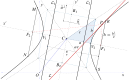
\includegraphics{hiperbola} 

}

\caption{Hipérbola}\label{fig:hiperbola}
\end{figure}

\[\frac{d\left[P;F_1\right]}{d\left[P;\mathcal{L}_1\right]}=e=\frac{d\left[P;F_2\right]}{d\left[P;\mathcal{L}_2\right]}\]

\(c=ae\); \(d\left[C;\mathcal{L}_1\right]=d\left[C;\mathcal{L}_2\right]=\frac{a}{e}\) y \(e>1\); en efecto \[\frac{d\left[R;F_1\right]}{d\left[R;\mathcal{L}_1\right]}=\frac{\frac{b^2}{a}}{c-d\left[C;\mathcal{L}_1\right]}=\frac{c^2-a^2}{a(c-d\left[C;\mathcal{L}_1\right])}\]

\[\frac{d\left[V_2;F_1\right]}{d\left[V_2;\mathcal{L}_1\right]}=\frac{c-a}{a-d\left[C;\mathcal{L}_2\right]}.\]

De la primera \[d\left[C;\mathcal{L}_2\right]=a-\frac{c-a}{e}\implies c-d\left[C;\mathcal{L}_2\right]=a-\frac{(c-a)(e+1)}{e}.\]

De la segunda ecuación \[c^2-a^2=ae\frac{(c-a)(e+1)}{e}\implies c+a=a(e+1)\implies c=ae\] luego \(d\left[C;\mathcal{L}_2\right]=a-\frac{(c-a)(ae+a)}{e}=\frac{a}{e}\) y el caso \(d\left[C;\mathcal{L}_1\right]\) es similar. Finalmente \(e=\frac{c}{a}>1\) pues \(0<a<c.\)

\(P=(x,y)=C+x'\vec{u}+y'\vec{u}^\perp\) \(x'=[(x,y)-C]\vec{u}\) y \(y'=[(x,y)-C]\vec{u}^\perp\)

\(F_1=C+c\vec{u}\) y \(F_2=C-c\vec{u}\) tambien \(V_1=C+a\vec{u}\) y \(V_2=C-a\vec{u}\) entonces \[\frac{d\left[P;F_1\right]}{d\left[P;\mathcal{L}_1\right]}=e\iff d\left[P;F_1\right]^2=e^2d\left[P;\mathcal{L}_1\right]^2\] haciendo uso de \(c=ae\) y \(c^2=a^2+b^2\) se tiene lo siguiente

\[(x'-c)^2+y'^2=e^2\left(x'-\left(\frac{a}{e}\right)\right)^2\]

\[(c^2-a^2) x'^2+a^2y'^2=a^2(c^2-a^2)\]

\[b^2x'^2-a^2y'^2=a^2b^2\]

De este modo \(P\in\mathcal{H}\) si \(P\) satisface la ecuación vectorial \[P=(x,y)=V+x'\vec{u}+y'\vec{u}^\perp;\: \text{donde } \frac{x'^2}{a^2}-\frac{y'^2}{b^2}=1; \:\left|\vec{u}\right|=1.\]

Cuando el eje es paralelo al eje \(X\); \(\vec{u}=i=(1,0)\) entonces \[(x,y)=V+x'\vec{u}+y'\vec{u}^\perp=(h+x',k+y')\] se tiene \(x'=x-h\) y \(y'=y-k\) en \(\frac{x'^2}{a^2}-\frac{y'^2}{b^2}=1\); resulta \[\frac{(y-k)^2}{a^2}-\frac{(y-k)^2}{b^2}=1\] entonces \(F_1=C+c\vec{u}=(h-\frac{a}{e},k)\) y \(F_2=C+c\vec{u}=(h-\frac{a}{e},k)\); \(\mathcal{L}_1: x=h-\frac{a}{e}\) y \(\mathcal{L}_2: x=h+\frac{a}{e}\) y las asíntotas de \(y'=\pm\frac{a}{b}x'\) se convierte en \((y-k)=\pm\frac{a}{b}(x-h)\). Además \(\frac{x^2}{a^2}-\frac{y^2}{b^2}=1\); si \(V\) está en el origen.

Cuando el eje es paralelo al eje \(Y\); \(\vec{u}=j=(0,1)\) se tiene \[(x,y)=V+x'\vec{u}+y'\vec{u}^\perp=(h-y',k+x')\] implica que \(x'=y-k\) y \(y'=h-x\) en \(\frac{x'^2}{a^2}-\frac{y'^2}{b^2}=1\); resulta \[\frac{(y-k)^2}{a^2}-\frac{(y-k)^2}{b^2}=1\] entonces \(F_1=C+c\vec{u}=(h+c,k)\); \(\mathcal{L}_1: x=k+\frac{a}{e}\) y \(\mathcal{L}_2: x=k-\frac{a}{e}\) y las asíntotas de \(y'=\pm\frac{b}{a}x'\) se convierte en \((y-k)=\pm\frac{b}{a}(x-h)\). Además \(\frac{x^2}{a^2}-\frac{y^2}{b^2}=1\); si \(V\) está en el origen.

\citep{vincze2014college}
\#\# Ejercicios

\hypertarget{appendix-apendice}{%
\appendix \addcontentsline{toc}{chapter}{\appendixname}}


\hypertarget{ecuaciones-de-primer-grado}{%
\chapter{Ecuaciones de primer grado}\label{ecuaciones-de-primer-grado}}

\citep{xie2015}

\hypertarget{raices-de-una-ecuacion-de-segundo-grado}{%
\section{Raices de una ecuacion de segundo grado}\label{raices-de-una-ecuacion-de-segundo-grado}}

\hypertarget{propiedades-de-una-ecuacion-de-segundo-grado}{%
\section{Propiedades de una ecuacion de segundo grado}\label{propiedades-de-una-ecuacion-de-segundo-grado}}

\hypertarget{ecacuaciones-lineales-de-primer-grado}{%
\chapter{Ecacuaciones lineales de primer grado}\label{ecacuaciones-lineales-de-primer-grado}}

\hypertarget{soluciones-de-ecuacuiones-lineales-de-primer-grado}{%
\section{Soluciones de ecuacuiones lineales de primer grado}\label{soluciones-de-ecuacuiones-lineales-de-primer-grado}}

\hypertarget{soluciones}{%
\section{Soluciones \ldots{}}\label{soluciones}}

\hypertarget{forma-matricial-de-una-ecuaciuxf3n-lineal}{%
\section{Forma matricial de una ecuación lineal}\label{forma-matricial-de-una-ecuaciuxf3n-lineal}}

\bibliography{book.bib,packages.bib}

\printindex

\end{document}
